\section{Produktbeschreibung und Funktion}

Aufgrund der Resultate der Evaluation der Lösungsprinzipien wurde beschlossen, 
das Konzept der stationären Abschussvorrichtung (Drehturm) weiter 
auszuarbeiten. 

Hierbei handelt es sich um ein nicht fahrbares, autonom arbeitendes Gerät mit 
einer in horizontaler Richtung drehbaren Abschussvorrichtung. Der gesamte Aufbau 
des Abschussmechanismus inklusive Balllager befindet sich auf einer drehbaren 
Plattform, welche auf einem geeignetem Stativ platziert ist. Die Plattform 
wird durch einen Schrittmotor und eine Zahnradübersetzung präzise in Position 
gebracht. Der Abschusswinkel in vertikaler Richtung ist hierbei fixiert. 

Die Abschussvorrichtung besteht im wesentlichen aus einem Balllager, einer 
Ballnachführung und einem sich schnell drehenden Rad, welches die Bälle auf 
die gewünschte Abschussgeschwindigkeit beschleunigt. Die Bauweise dieser drei 
Komponenten soll integral erfolgen, wobei das längliche, Quaderförmige 
Balllager als Hauptstruktur dient. An diesem sind sowohl das Rad für die 
Ballbeschleunigung als auch die Komponenten der Ballnachführung befestigt.

\subsection{Drehvorrichtung}
Das unterste Element des Gerätes besteht aus einer kleinen, möglichst leichten 
Bodenplatte. An dieser Bodenplatte werden 4 Beine (Rohrform) angeschraubt. Mit 
zwei Axial-Kugellagern wird ein grosses Zahnrad (z1=120) auf der Bodenplatte 
befestigt. Auf dieses wird dann der gesamte Aufbau bestehend aus Stativ, 
Balllagerung und Abschussvorrichtung montiert. 

\begin{figure}[h!]          
	\centering             
	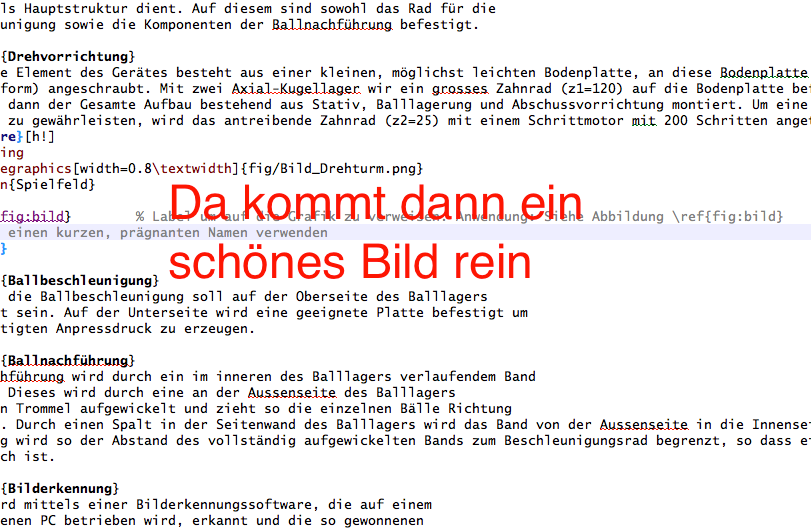
\includegraphics[width=0.8\textwidth]{fig/Bild_Drehturm.png}    
	\caption{Drehturm}
	
	\label{fig:bild}        % Label um auf die Grafik zu verweisen. Anwendung: Siehe Abbildung \ref{fig:bild}
	% Bitte einen kurzen, prägnanten Namen verwenden
\end{figure}

Um eine genaue Ausrichtung zu gewährleisten, wird das antreibende Zahnrad 
(z2=25) mit einem Schrittmotor mit 200 Schritten angetrieben (QSH 4218, 
QMot.eu). Bei 200 Schritten ergibt sich eine Genauigkeit von 1.8$^\circ$, mit einer 
Übersetzung von z1/z2=4.8 ergibt das eine Ausrichtgenauigkeit von 0.375$^\circ$. Dies 
bedeutet für eine Distanz von 1900mm eine seitliche Abweichung von 
$1900 \cdot \tan(0.375^\circ)= 12.5mm$. Somit wird diese Abweichung bei einem 
Korbdurchmessen von 30cm keine Rolle spielen. Des weiteren wird mit einem 
geeigneten Treiber sogar noch eine höhere Genauigkeit erreicht 
(Zwischenschritte), welche jedoch vom Drehmoment abhängig ist. 

\subsection{Ballbeschleunigung}
Das Rad für die Ballbeschleunigung soll auf der Oberseite des Balllagers 
positioniert sein. Auf der Unterseite wird eine geeignete Platte befestigt um 
so den benötigten Anpressdruck zu erzeugen. 

\subsection{Ballnachführung}
Die Ballnachführung wird durch ein im Inneren des Balllagers verlaufendes Band 
realisiert. Dieses wird durch eine an der Aussenseite des Balllagers 
angebrachten Trommel aufgewickelt und zieht so die einzelnen Bälle in Richtung 
Abschussrad. Durch einen Spalt in der Seitenwand des Balllagers wird das Band 
von der Aussenseite in die Innenseite geführt. Gleichzeitig wird so der 
Abstand des vollständig aufgewickelten Bands zum Beschleunigungsrad begrenzt, 
so dass ein Verklemmen nicht möglich ist.

\subsection{Bilderkennung}
Der Korb wird mittels einer Bilderkennungssoftware, die auf einem 
angeschlossenen PC betrieben wird, erkannt und die so gewonnenen 
Positionsdaten an die entsprechenden Ansteuerungskomponenten gesendet. Diese 
können anschliessend den Winkel in horizontaler Richtung, sowie die 
Abschussgeschwindigkeit und somit die Abschussgeschwindigkeit, mit der Drehzahl des 
Beschleunigungsrades regeln.

\subsection{Signalübertragung}
Die Übertragung des Startsignals, sowie die Anzeige des Endsignals erfolgt per 
WLAN über einen zweiten Laptop.
